\section{Parallele Architekturen}

\begin{compactitem}
\item Architektur eines einzelnen Prozessors
\item Infrastruktur über mehrere Prozessoren hinweg
\end{compactitem}

\subsection{Single Chip}

Da die Performance der Taktraten eines Prozessors pro Jahr ungefähr um 30\%
steigt, die Performance von Applikationen aber um 55\% - 75\% pro Jahr steigt,
kann die Taktrate nicht alleine für den Speedup herangezogen werden.

\subsection{Vier Ebenen von Parallelität}

\begin{compactitem}
\item auf Bitebene
\item Pipelining
\item auf der Ebene von Funktionalen Einheiten (ALU, FPU, etc.)
\item Prozess- und Threadebene
\end{compactitem}

\subsubsection{Die Bitebene}

Mit der Bitebene sind die Algorithmen gemeint, welche z.B. bei den Carry-Look-Ahead
Addern benützt werden. Diese Effizienzsteigerungen werden durch Parallelität anstatt
durch Sequentielles Addieren erreicht. Grundsätzlich können alle Bits in einem 
(Register) Word parallelisiert werden. Da die maximale Größe der ansteuerbaren
Adressen fürs erste so hoch ist, dass man jetzt noch nicht daran denkt, diese
jemals auszuschöpfen, ist die Entwicklung bei 64 Bit Wörtern stehen geblieben.

\subsubsection{Pipelining}

Pipelining nützt die Tatsache aus, dass jede Instruktion auf einem Prozessor
mehrere Schritte hat. Fetch, Decode, Execute und Write-back. Traditionelle
Prozessoren haben diese Schritte Sequentiell bearbeitet. Wichtig hierbei ist
die Tatsache, dass die Instruktionen voneinander unabhängig sind und keine
Abhängigkeiten besitzten. So darf I1 nicht einen Wert berechnen, den I2 (die
nächste Instruktion) für die Ausführung benötigt. Unter diesen Voraussetzungen
können die Teilaufgaben parallelisiert werden, da die Ressourcen des Prozessors
unterschiedlich benützt werden in den einzelnen Teilaufgaben.

\begin{center}
	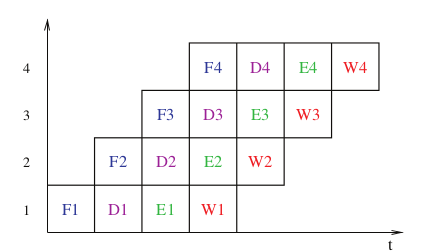
\includegraphics[width=1.00\linewidth]{pipelining.png}
	\captionof{figure}{Nach oben Instruktionen, nach Rechts die Zeit}
\end{center}

Die Geschwindigkeitssteigerung erhöht sich mit der Anzahl der Instruktionen.
Das Verfahren ist besonders effizient, wenn die Instruktionen alle ungefähr die
gleiche Zeit benötigen, somit kommt es nicht zu NOP-Rutschen wegen ungleichen 
Längen. Prozessoren mit vielen Stages (Teilaufgaben) nennt man \textit{super-pipelined}.
Beschränkungen sind natürlich die Abhängigkeiten untereinander und Instruktionen
können nicht beliebig weit geteilt werden.

\subsubsection{Funktionale Einheiten}
Auch funktionale Einheiten wie ALUs oder FPUs können parallel arbeiten. Im Prinzip
gibt es zwei Herangehensweisen für die Parallelisierung. Die \textbf{statische}
Variante wird von VLIW (= Very Long Instruction Word) benützt (z. B. IA 64). 
Der Compiler generiert bereits Maschinencode, der die einzelnen funktionalen
Einheiten mappt. Die Instruktionswörter haben variable Länge (daher der Name).
Der andere Ansatz ist die \textbf{dynamische} bei superskalaren Prozessoren (wie dem i7). 
Eine automatische Laufzeitanalyse mappt zur Laufzeit den Maschinencode zu den 
einzelnen Funktionalen Einheiten. Als Hinweis: Moderne Prozessoren erlauben
2 bis 6 parallele Instruktionen in den funktionalen Einheiten.

Dynamische Scheduling kostet einen großen Overhead (z. B. in der Chipgröße), jedoch
sind Superskalare Prozessoren heute \textbf{State of the Art}. Auf den meisten
Prozessoren können nicht mehr als 4 Instruktionen des gleichen Typs dispatcht werden.
Die dekodierten Instruktionen werden in dem Instruktion-Fenster gespeichert und
werden an die Funktionalen Einheiten versandt sobald die Operanden verfügbar sind.
Wichtig ist vorallem die Korrektheit: Parallele Verarbeitung darf nicht die
Semantik des Codes zerstören. Dies wird durch den \textbf{Reorder Buffer} garantiert.
Schreiboperationen auf Register werden nicht ausgeführt solange bis alle vorher 
gehenden Operationen, welche auf die selben Register schreiben, nicht beendet wurden.
In der Tomasulo Architektur wird das durch den zusätzlichen Stage \textit{Commit}
erreicht.
\subsubsection{Prozesse und Threads}


\section{Klassifikation von Parrallelcomputern}

\subsection{M. Flynns Klassifikation}

\subsubsection{SISD}
\subsubsection{MISD}
\subsubsection{SIMD}
\subsubsection{MIMD}

\subsection{Klassifikation nach Memory Layout}
